% Repacked from paper-section-en-final.md (2026-07-06). Content is sections
% 5-7 of the full paper; section counter is offset below so numbering
% matches the source. Front matter (title/author) is placeholder only --
% it is not part of the source content and must be filled from the
% full-paper manuscript before submission.
\documentclass[sigconf,review]{acmart}

\usepackage[T1,T2A]{fontenc}
\usepackage[russian,english]{babel}
\usepackage{amsmath}
\usepackage{booktabs}
\usepackage{filecontents}

% --- Metric macros (terminology-spec.md, 2026-07-06 naming) -----------------
% Old internal codes (M1/M2/M3, P1/P2/P3, R-T0/T1/T2) must never appear
% below this line; use these macros everywhere a metric symbol is needed.
\newcommand{\Rdoc}{\ensuremath{R_{\mathrm{doc}}}}
\newcommand{\Rspan}{\ensuremath{R_{\mathrm{span}}}}
\newcommand{\Rstrict}{\ensuremath{R_{\mathrm{strict}}}}
\newcommand{\Rall}{\ensuremath{R_{\mathrm{all}}}}
\newcommand{\Rclean}{\ensuremath{R_{\mathrm{clean}}}}
\newcommand{\Rterm}{\ensuremath{R_{\mathrm{term}}}}
\newcommand{\Pmention}{\ensuremath{P_{\mathrm{mention}}}}
\newcommand{\Ptype}{\ensuremath{P_{\mathrm{type}}}}
\newcommand{\Plabel}{\ensuremath{P_{\mathrm{label}}}}

% --- Bibliography ------------------------------------------------------
% NOTE: paper-section-en-final.md contains NO BibTeX block -- only bracketed
% author/year mentions inline (e.g. "[Botha et al. 2020]"). The entries
% below were reconstructed from those in-text mentions solely to resolve
% every \cite key used in Related Work. All 7 entries verified 2026-07-06
% against ACL Anthology / arXiv / OpenReview / ACM DL (authors, titles,
% venues, pages).
\begin{filecontents*}[overwrite]{references.bib}
@inproceedings{botha2020mewsli,
  author    = {Botha, Jan A. and Shan, Zifei and Gillick, Daniel},
  title     = {Entity Linking in 100 Languages},
  booktitle = {Proceedings of the 2020 Conference on Empirical Methods in Natural Language Processing (EMNLP)},
  year      = {2020},
  address   = {Online},
  publisher = {Association for Computational Linguistics},
  pages     = {7833--7845},
  doi       = {10.18653/v1/2020.emnlp-main.630}
}

@article{decao2022mgenre,
  author  = {De Cao, Nicola and Wu, Ledell and Popat, Kashyap and Artetxe, Mikel and Goyal, Naman and Plekhanov, Mikhail and Zettlemoyer, Luke and Cancedda, Nicola and Riedel, Sebastian and Petroni, Fabio},
  title   = {Multilingual Autoregressive Entity Linking},
  journal = {Transactions of the Association for Computational Linguistics},
  volume  = {10},
  pages   = {274--290},
  year    = {2022},
  publisher = {MIT Press},
  doi     = {10.1162/tacl\_a\_00460}
}

@inproceedings{decao2021genre,
  author    = {De Cao, Nicola and Izacard, Gautier and Riedel, Sebastian and Petroni, Fabio},
  title     = {Autoregressive Entity Retrieval},
  booktitle = {International Conference on Learning Representations (ICLR)},
  year      = {2021},
  url       = {https://openreview.net/forum?id=5k8F6UU39V}
}

% arXiv-only preprint: positively ruled out of DLnLD@LREC-COLING-2024; no
% peer-reviewed venue found as of 2026-07-06.
@misc{damuel2023,
  author = {Kube\v{s}a, David and Straka, Milan},
  title  = {{DaMuEL}: A Large Multilingual Dataset for Entity Linking},
  year   = {2023},
  eprint = {2306.09288},
  archivePrefix = {arXiv}
}

@inproceedings{gerlach2021,
  author    = {Gerlach, Martin and Miller, Marshall and Ho, Rita and Harlan, Kosta and Difallah, Djellel},
  title     = {Multilingual Entity Linking System for Wikipedia with a Machine-in-the-Loop Approach},
  booktitle = {Proceedings of the 30th ACM International Conference on Information and Knowledge Management (CIKM)},
  year      = {2021},
  pages     = {3818--3827},
  doi       = {10.1145/3459637.3481939}
}

@inproceedings{conia2024kgmt,
  author    = {Conia, Simone and Lee, Daniel and Li, Min and Minhas, Umar Farooq and Potdar, Saloni and Li, Yunyao},
  title     = {Towards Cross-Cultural Machine Translation with Retrieval-Augmented Generation from Multilingual Knowledge Graphs},
  booktitle = {Proceedings of the 2024 Conference on Empirical Methods in Natural Language Processing (EMNLP)},
  year      = {2024},
  address   = {Miami, Florida, USA},
  publisher = {Association for Computational Linguistics},
  pages     = {16343--16360}
}

@inproceedings{semeval2025eamt,
  author    = {Conia, Simone and Li, Min and Navigli, Roberto and Potdar, Saloni},
  title     = {{SemEval}-2025 Task 2: Entity-Aware Machine Translation},
  booktitle = {Proceedings of the 19th International Workshop on Semantic Evaluation (SemEval-2025)},
  year      = {2025},
  address   = {Vienna, Austria},
  publisher = {Association for Computational Linguistics},
  pages     = {2535--2557}
}
\end{filecontents*}

% Placeholder front matter -- not present in the source section; fill from
% the full-paper manuscript.
\acmConference[Conf'26]{TODO: full-paper venue}{TODO: dates}{TODO: location}
\settopmatter{printacmref=false} % suppress the ACM reference/copyright block (no camera-ready rights info yet)
% \footnotetextcopyrightpermission is a documented acmart internal used in several
% acmart-based repos to blank the copyright-permission footnote alongside the line
% above; left in place but UNVERIFIED against an actual acmart.cls (no toolchain in
% this container) -- if compilation reports it undefined, delete this line only,
% \settopmatter above is independently sufficient.
\renewcommand\footnotetextcopyrightpermission[1]{}

\begin{document}

\title{TODO: full-paper title (this file contains only \S5--\S7)}
\author{TODO: author list}
\affiliation{%
  \institution{TODO: affiliation}
  \country{TODO: country}
}
\email{TODO@example.org}

\maketitle

\setcounter{section}{4} % first \section below renders as "5", matching the source

\section{Evaluation}
\label{sec:evaluation}

We ask one question that standard entity-linking benchmarks leave open: given
no task supervision, how well can a system find the domain terms in a Russian
text and ground each to the right Wikidata entity? The multilingual linking
suites that would seem to answer it do not. Mewsli-9 and its successors span a
hundred languages but not Russian, and every strong number on them comes from a
linker trained on millions of the same Wikipedia anchors it is scored against.
We are after the opposite regime: a zero-shot pipeline, run on Russian
historical prose, measured at the point where a mention is found and resolved
rather than through downstream translation quality. This section builds a
reference benchmark for that regime and reports where the difficulty actually
lies.

\subsection{Benchmark construction}
\label{sec:benchmark-construction}

We derive the reference set from a resource Wikipedia editors have already
produced: the internal links they place by hand in article bodies. Each
body-paragraph link whose target resolves to a Wikidata item yields one
\emph{gold mention}: a tuple of token index, surface form, QID, and span
length. Resolution follows redirect chains through the MediaWiki API with no
learned component, so the benchmark is deterministic and rebuilds bit-for-bit
from a cached HTML snapshot of each article. We remove links to chronology
targets (years, decades, centuries, identified by the target's
\emph{instance-of} class), which annotate temporal navigation rather than
terminology. The corpus of 100 articles yields 8,829 in-text links; 405 are
chronology-filtered and 6 carry no Wikidata item, leaving \textbf{7,959 gold
mentions over 3,868 distinct QIDs}.

The 100 articles come in ten thematic sections of ten (Sumer, Egypt, Assyria,
the Hittite kingdom, Phoenicia, Achaemenid Iran, India, China, Greece, Rome).
Within each section we shuffle the category subtree under a fixed seed, walk it
in order, and admit an article only when it clears a deterministic gate: at
least thirty unique body links, an earliest Wikidata date before 500~CE
(undated pages kept), and a short \emph{instance-of} blacklist for off-topic
media. We stop at ten admissions. The corpus is fixed by seed and gate, not
curated by hand.

One property of this reference set shapes every metric that follows.
Wikipedia's style guide asks editors to link an entity at its first mention and
not again, and it never guarantees that every term in a passage is linked at
all. The annotations are precise where they exist but systematically
incomplete; a missing link is not evidence that a mention is not a term. We
therefore treat \textbf{recall as the primary axis}, the share of genuinely
annotated concepts a system recovers, and read precision only as a conservative
lower bound: a prediction absent from the reference may be correct rather than
wrong.

\subsection{Metrics}
\label{sec:metrics}

Our headline metric is \textbf{document-level recall} (\Rdoc): a gold mention
counts as recovered if its QID appears anywhere in the system's predictions
for that article. This states the task in its most transparent form: the
article's concept was found and grounded to the right entity. It is robust to
tokenisation and mention-boundary disagreements. Two positional variants bound
it from below and appear only in the matching-strictness ablation:
\textbf{strict-match recall} (\Rstrict) demands an equal first-token index,
normalised surface, and QID; \textbf{span-overlap recall} (\Rspan) requires
overlapping spans and an equal QID. \Rstrict\ $\le$ \Rspan\ $\le$ \Rdoc\ holds
on every run.

We report precision under span-overlap matching in three readings, each a
tighter lower bound than the last. \textbf{Mention-level precision}
(\Pmention) scores every QID-bearing prediction. \textbf{Type-level precision}
(\Ptype) first deduplicates predictions by normalised surface and QID, which
offsets the do-not-relink convention; the gap between the two measures that
convention directly. \textbf{Label-verified precision} (\Plabel) further
credits a prediction absent from the reference when its surface exists as a
Wikidata label; we report it excluding the deterministic exact-label path,
where the surface is a label by construction. Every reported cell carries a
Wilson 95\% interval, and cells with fewer than thirty gold mentions are
flagged and never interpreted.

A large gap between capitalised and lowercase reference mentions, reported in
\S\ref{sec:results}, raises a question about the reference itself: is some of
it not terminology at all? To answer it deterministically we define three
nested \textbf{gold-filtering tiers} on properties of each target QID. \Rall\
is the unfiltered set. \Rclean\ removes structural noise: the meta and
calendar pages that survive earlier filters. \Rterm\ further removes generic
lexical classes that a terminology task should not reward: languages and
scripts, taxa and materials, units and standards, academic and abstract
concepts. A target is dropped only when \emph{every} one of its
\emph{instance-of} classes maps to a noise bucket, which protects multi-typed
real entities.

\subsection{System under test}
\label{sec:system-under-test}

The system under test is a deterministic-first grounding pipeline
(Figure~\ref{fig:pipeline}). An LLM extractor proposes mentions paragraph by
paragraph. A candidate ladder then queries Wikidata by lemma, then by
surface, with full-text and title-sitelink fallbacks when a rung returns
nothing. A single exact match against a candidate's label or alias resolves
the mention deterministically, with no LLM involvement; genuine ambiguity
escalates to an LLM judge that must pick among the retrieved candidates or
abstain. The pipeline never silently falls back to a top-ranked guess. A
three-component ablation over the ladder (lemma search, search fallbacks,
alias matching), run on a 20-article subset of 1,443 gold mentions and
cross-checked against an independent 91-term set, attributes +0.322
span-overlap recall to lemma search and +0.145 to search fallbacks over the
all-off baseline; alias matching adds no measurable accuracy (+0.004) and is
kept only for decision-trace transparency. The same candidate model serves as
both extractor and judge, and the ladder configuration is fixed for the main
runs.

\begin{figure}
  \centering
  % figure asset: drafts/g6-pipeline.(svg->png/pdf), generated separately
  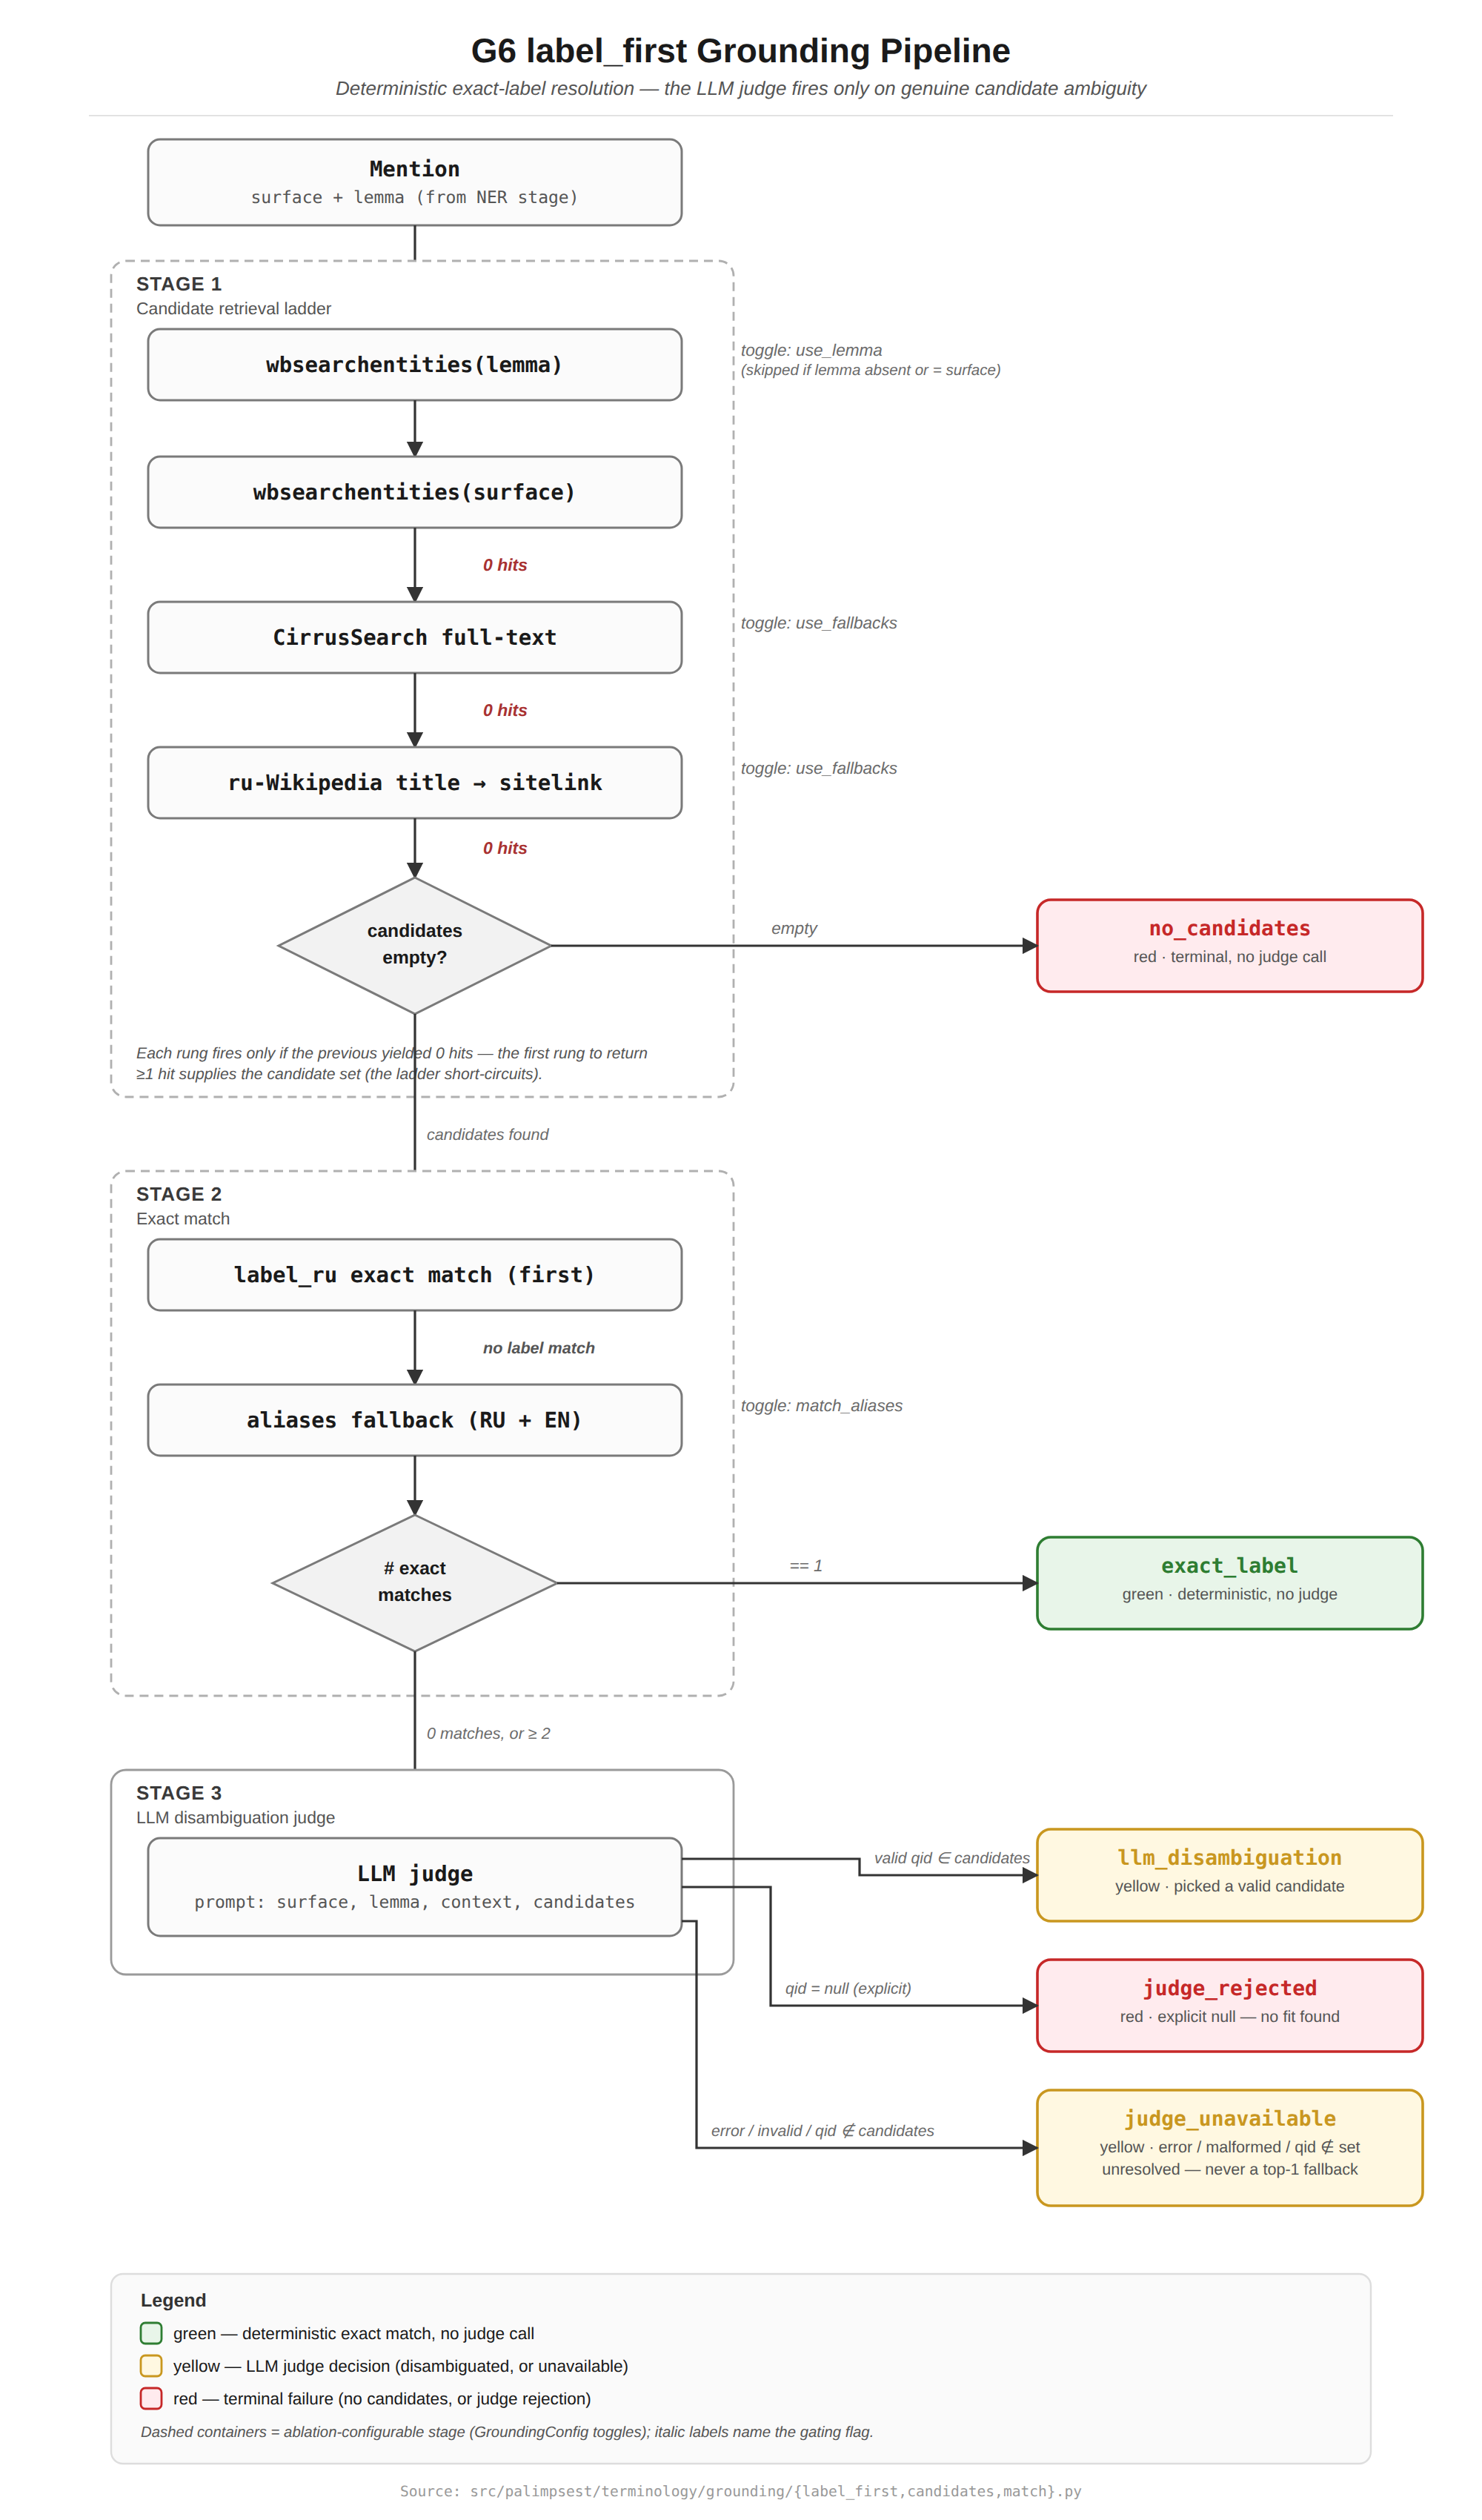
\includegraphics[width=\linewidth]{g6-pipeline}
  \caption{The deterministic-first grounding pipeline: LLM mention
  extraction, a candidate ladder over Wikidata (lemma, surface, full-text and
  title-sitelink fallbacks), a deterministic exact-label match, and an LLM
  judge for genuine ambiguity.}
  \label{fig:pipeline}
\end{figure}

\section{Results and Analysis}
\label{sec:results}

\begin{table}
  \caption{Full-corpus results (100 articles, 7,959 gold mentions): recall in
  three matching modes, precision under span-overlap matching, Wilson 95\%
  intervals on \Rdoc.}
  \label{tab:main}
  \begin{tabular}{lrrrrrr}
    \toprule
    Model & \Rdoc\ [95\% CI] & \Rspan & \Rstrict & \Pmention & \Ptype & Gold mentions \\
    \midrule
    gemini-3.1-flash-lite & \textbf{0.690} [0.680--0.700] & 0.630 & 0.610 & 0.300 & 0.451 & 7,959 \\
    deepseek-v4-flash     & \textbf{0.614} [0.604--0.625] & 0.524 & 0.509 & 0.305 & 0.458 & 7,959 \\
    qwen3.7-plus          & --- & --- & --- & --- & --- & 7,959 \\
    % TODO(qwen): fill from report --p3
    \bottomrule
  \end{tabular}
\end{table}

On document-level recall, gemini-3.1-flash-lite reaches 0.690 and
deepseek-v4-flash 0.614, with narrow intervals over 7,959 gold mentions.
Precision sits near 0.30 at the mention level and near 0.45 at the type level
for both models; the type gain is exactly the do-not-relink convention made
visible. Label-verified precision, which credits a further class of
unmatched-but-valid predictions, reaches 0.526 for gemini-3.1-flash-lite and
0.530 for deepseek-v4-flash, about 0.07 above type-level precision for both
models and, like grounding accuracy, nearly identical across models.

\textbf{The recall gap has a single, clean cause.} We decompose recall at each
gold position into two factors: \emph{extraction coverage}, whether the
pipeline produced any resolved prediction at that position, and
\emph{grounding accuracy}, whether that prediction carried the right QID.
Coverage separates the models sharply: 0.763 for gemini against 0.632 for
deepseek. Grounding accuracy does not move: \textbf{0.814 and 0.815, identical
to the third decimal}. The entire recall difference lives in the extraction
stage. Given a mention, both models ground it about equally well, and well in
absolute terms: accuracy runs 0.92--0.93 on the deterministic exact-label path
and 0.85--0.86 on judge-disambiguated cases, with the residual conditional
loss concentrated in explicit abstentions, roughly 7--8\% of covered
positions. This is the result to carry out of the section. The bottleneck is
finding the terms, not linking them.

\textbf{The mention-type slice points to the same place.} Document recall on
capitalised mentions reaches 0.828 for gemini but only \textbf{0.414 on
lowercase terminology} (type assigned by surface capitalisation). Common-noun
terms, not proper names, are where coverage fails. The gap is wide enough to
ask whether the lowercase reference is really terminology or partly annotation
noise, and we test that with the gold-filtering tiers (Table~\ref{tab:tiers}).
The answer is: partly. Of the 1,551 unmatched lowercase mentions, about
\textbf{34\% are filterable noise} (language glosses such as
\foreignlanguage{russian}{англ.} and \foreignlanguage{russian}{др.-греч.},
taxa, meta pages, academic labels) and about \textbf{66\% are genuine domain
terms the model misses} (\foreignlanguage{russian}{мумия},
\foreignlanguage{russian}{папирус}, \foreignlanguage{russian}{зиккурат},
cylinder seal, satrap). Cleaning the reference lifts gemini's terminology
recall from 0.414 to 0.474 and its overall recall from 0.690 to 0.741, yet the
capitalised/lowercase gap barely narrows (0.841 against 0.474 at \Rterm). The
deficit is a property of the extractor, not of the annotation, and the model
ranking is unchanged across all three tiers.

\begin{table}
  \caption{Candidate-ladder ablation (20-article subset, 1,443 gold
  mentions). Rows enable lemma search, search fallbacks, and alias matching
  (bit codes noted below).}
  \label{tab:ablation}
  \begin{tabular}{lrrr}
    \toprule
    Components enabled & \Rstrict & \Rspan & \Rdoc \\
    \midrule
    none                & 0.280 & 0.286 & 0.416 \\
    +aliases            & 0.283 & 0.290 & 0.422 \\
    +fallbacks          & 0.419 & 0.431 & 0.545 \\
    +fallbacks +aliases & 0.422 & 0.435 & 0.550 \\
    +lemma              & 0.593 & 0.608 & 0.683 \\
    +lemma +aliases     & 0.606 & 0.624 & 0.701 \\
    +lemma +fallbacks   & 0.608 & 0.624 & 0.699 \\
    \textbf{all}        & \textbf{0.622} & \textbf{0.640} & \textbf{0.717} \\
    \bottomrule
  \end{tabular}

  \smallskip
  {\footnotesize Configurations 000--111 over (lemma, fallbacks, aliases);
  the all-components row is labeled ``all''.\par}
\end{table}

The ladder ablation explains where recall comes from. Lemma search is the
dominant lever: adding it alone lifts span-overlap recall from 0.286 to 0.608,
and removing it from the full configuration costs 0.204. Search fallbacks help
most in isolation (+0.145) but only marginally once lemma search is present
(+0.016), because lemma search already reaches most of the terms the
full-text fallback was there to recover. Alias matching moves nothing
measurable and earns its place only in the decision trace.

\begin{table}
  \caption{Gold-filtering tiers (\Rdoc). The lowercase column gives gemini's
  recall on the surviving lowercase mentions.}
  \label{tab:tiers}
  \begin{tabular}{lrrrr}
    \toprule
    Tier & Gold mentions & gemini \Rdoc & deepseek \Rdoc & gemini \Rdoc\ (lowercase) \\
    \midrule
    \Rall\ (raw) & 7,959 & 0.690 & 0.614 & 0.414 \\
    \Rclean      & 7,796 & 0.704 & 0.627 & 0.434 \\
    \Rterm       & 7,174 & \textbf{0.741} & \textbf{0.663} & \textbf{0.474} \\
    \bottomrule
  \end{tabular}
\end{table}

\begin{table}
  \caption{Per-section recall (\Rdoc).}
  \label{tab:persection}
  \begin{tabular}{lrrr}
    \toprule
    Section & gemini & deepseek & Gold mentions \\
    \midrule
    sumer            & 0.781 & 0.662 & 613 \\
    assyria          & 0.767 & 0.638 & 879 \\
    hittite          & 0.735 & 0.461 & 649 \\
    achaemenid\_iran & 0.719 & 0.684 & 713 \\
    india            & 0.689 & 0.649 & 843 \\
    greece           & 0.645 & 0.598 & 1,506 \\
    rome             & 0.633 & 0.605 & 683 \\
    egypt            & 0.584 & 0.499 & 579 \\
    china            & 0.581 & 0.467 & 458 \\
    phoenicia        & 0.551 & 0.488 & 1,036 \\
    \bottomrule
  \end{tabular}
\end{table}

Per-section recall shows the stronger model is also the steadier one. Gemini
ranges from 0.551 on Phoenicia to 0.781 on Sumer; deepseek swings wider, 0.461
to 0.684. Deepseek's worst section partly reflects paragraphs lost to
transient failures during its run (4.1\% of the corpus, declared in run
metadata and worth about 0.02 recall if corrected), but the gap to gemini
survives that correction. The difference is genuine per-domain weakness, not
an availability artifact.

\textbf{Evaluation integrity.} One rung of the candidate ladder deserves
explicit scrutiny, because it reuses the exact mapping the reference is built
from. The title-sitelink fallback resolves a Russian Wikipedia title to a QID
through the same \emph{pageprops} path that turns a human wikilink into a
gold mention, so any recall it contributes is partly circular by
construction. We quantified it by replaying the ladder offline from each
run's own cache. The rung supplies about 1\% of grounded predictions (1.22\%
for gemini, 1.04\% for deepseek), and those predictions match the reference
at 52--60\%, far above what a random 1\% share would yield: the circularity
is real, not coincidental. Its net effect on the headline is small. Removing
the rung costs 0.5--0.8 recall points across both models, both matching
modes, and both tiers, and it does not explain the gemini/deepseek gap, which
both models pay about equally. The reported runs predate this finding and
include the rung; we disable it in the evaluation protocol going forward.

\textbf{Limitations.} Two caveats bound these numbers. Wikipedia's category
graph is noisy, and roughly three of the 100 articles fall outside the target
period; we disclose them rather than curate the corpus to its result. We
assign mention type by surface capitalisation alone, without
cross-tabulation against the extractor's own category, so the
capitalised/lowercase split is a proxy for proper-noun versus common-noun
terminology rather than a verified partition.

\section{Related Work}
\label{sec:related}

Building reference annotations from Wikipedia's own hyperlinks is
established practice. Mewsli-9~\citep{botha2020mewsli} extracts anchor texts
as linked mentions and resolves them to Wikidata across nine languages;
% TODO(verify): the 0.89--0.90 R@1 range could not be pinned to a source in
% the 2026-07-06 citation pass (mGENRE's 90.2 micro-accuracy IS confirmed).
supervised multilingual linkers reach 0.89--0.90 R@1 on it, with
mGENRE~\citep{decao2022mgenre} reporting 90.2 micro-accuracy. Neither covers
Russian, and both train on the very link distribution they are scored
against, so their numbers describe a supervised, in-distribution regime
rather than ours. The editorial convention behind these anchors, linking an
entity only at its first mention, is documented directly by
DaMuEL~\citep{damuel2023} and compounded across languages by cross-lingual
link sparsity~\citep{gerlach2021}. That convention is exactly what makes the
reference precise but incomplete, and what motivates our recall-primary
protocol with precision as a lower bound. End-to-end linkers on curated
English data, GENRE~\citep{decao2021genre} at 83.7 micro-F1 on AIDA among
them, are not comparable head-to-head: they report F1 on a complete
annotation in another language and domain.

Our task sits closest to entity-aware machine translation, where the
grounding stage is a means rather than the object of measurement.
KG-MT~\citet{conia2024kgmt} retrieves source entities from a multilingual
knowledge graph to improve name translation and scores that retrieval only
through downstream translation quality (M-ETA), a setting since
institutionalised by SemEval-2025 Task 2~\citep{semeval2025eamt}, whose best
data-free system reaches 71.7 M-ETA. We measure the same find-and-ground step
those systems rely on, but directly and reproducibly, against human
annotations, on Russian, where no comparable baseline exists. The
contribution is complementary to that line of work, not competitive with it.

\bibliographystyle{ACM-Reference-Format}
\bibliography{references}

\end{document}
